\documentclass[12pt]{article}

\usepackage[francais]{babel}
\usepackage[utf8]{inputenc}
\usepackage[T1]{fontenc}
\usepackage[left=2cm,right=2cm,top=2cm,bottom=2cm]{geometry}
\usepackage{graphicx}

\begin{document}
\begin{titlepage}

\newcommand{\HRule}{\rule{\linewidth}{0.5mm}}

\center

\textsc{\LARGE Université de Rouen}\\[1.5cm]
\textsc{\Large Miniquiz}\\[0.5cm]
\textsc{\large Langage Web 1}\\[0.5cm]

\HRule \\[0.4cm]
{ \huge \bfseries Rapport De Projet}\\[0.2cm]
\HRule \\[1.5cm]

  \begin{minipage}{0.4\textwidth}
    \begin{flushleft} \large
      \emph{Membres:}\\
      Valentin \textsc{Crochemore}\\
      Yoann \textsc{Fleury}
    \end{flushleft}
  \end{minipage}
  ~
  \begin{minipage}{0.4\textwidth}
    \begin{flushright} \large
      \emph{Enseignant:} \\
      Florent \textsc{Nicart}
    \end{flushright}
  \end{minipage}\\[3cm]


  {\large Date : \today}\\[3cm]

  
\includegraphics{res/logo.png}\\[1cm]

  \vfill
\end{titlepage}

\newpage
\tableofcontents
\newpage

\section{Architecture Logicielle}
    \subsection{Base De Données}
        \paragraph{}
        L'architecture de notre base de données est la plus souple possible afin de permettre de futures extensions de l'application. On peut par exemple expliquer notre choix pour les tables suivantes :
        \begin{description}
            \item[mq\_access] Si l'application vient à évoluer, les droits d'accès ne sont pas codés en dur dans le code. Donc pour le moment, cette table contient deux lignes qui définissent l'administrateur et l'utilisateur normal, mais il est possible de rajouter par la suite un nouveau type d'utilisateur et d'ajouter des fonctions pour ceux-ci. Chaque rôle contient un identifiant numérique unique, une clef qui permet d'identifier plus simplement le rôle dans le code PHP et enfin, une brève description du rôle pour une meilleure compréhension de celui-ci.
            \item[mq\_answer] Nous avons choisi de stocker les réponses aux questions dans une table différente afin de pouvoir par la suite faire évoluer notre application en proposant plus de 4 réponses à chaque questions. Idem, on pourrait se servir de cette table pour proposer des réponses grâce à des requêtes AJAX et en fonction de la question, des réponses plausibles apparaissent aux yeux du créateur du quiz. Cette table stocke un identifiant numérique unique ainsi que le contenu de la réponse. Le contenu de la réponse peut contenir du Markdown qui sera interprété lors de l'affichage.
            \item[mq\_question] Comme son nom l'indique, cette table permet de stocker les questions. Elle est définie grâce à un identifiant numérique unique, la question sous format texte, et une colonne qui contient l'identifiant de la bonne réponse. Comme pour les réponses, le contenu de la question peut avoir du markdown qui sera interprété lors de l'affichage.
            \item[mq\_quiz] Cette table contient bien évidemment ce qui est lié à un quiz. C'est à dire un identifiant numérique unique, un titre de quiz, une description du quiz et enfin, l'identifiant numérique unique de l'utilisateur qui a créé le quiz.
            \item[mq\_quizsave] Comme son nom le laisse paraître, cette table stocke les sauvegardes des quiz. Un utilisateur peut dans notre application, s'il est connecté, faire un quiz et ne pas le terminer. A chaque question, l'état du quiz est sauvegardé. Cette table permet le stockage d'un identifiant numérique unique, de l'identifiant de l'utilisateur, du quiz qu'il a commencé et de la sauvegarde en JSON de l'état du quiz. Comme chaque quiz est différent dans son nombre de questions, une table générique n'était pas possible à mettre en place, d'où le choix du JSON pour la sauvegarde d'un quiz pour un utilisateur.
            \item[mq\_user] Cette table est assez basique pour stocker les utilisateurs. Elle permet de sauvegarder un identifiant numérique unique propre à chaque utilisateur, un login sous format texte, et un mot de passe haché grâce à l'algorithme \texttt{B\_CRYPT} qui fait parti de ces dernières conventions dans la sécurité web.
            \item[mq\_question\_answer] Cette table est une table de jointure qui permet de faire le lien entre une question et ses réponses. Quoi de plus basique pour une table de jointure que de contenir un identifiant numérique unique, l'identifiant numérique unique de la question et l'identifiant numérique unique de la réponse. Ainsi, à chaque ligne de cette table correspond une question avec une de ses réponses.
            \item[mq\_quiz\_question] Cette dernière table est également une table de jointure qui permet le lien entre un quiz et ses questions. Comme pour la table juste au dessus, quelque chose de basique qui contient un identifiant numérique unique pour la relation, un identifiant numérique unique définissant le quiz et enfin un identifiant numérique unique pour la question.
        \end{description}
    
    \subsection{Architecture MVC}
        \paragraph{Silex} L'avantage d'utiliser un framework dans un développement comme celui-ci, c'est qu'il force à utiliser de bonnes conventions de code et qu'il permet un code propre. Silex respecte des normes que nous avons également suivies, comme l'architecture MVC. Dans un premier temps, prenons la partie Controller qui est surement la plus importante dans notre projet. 
        
        \paragraph{Controller} Le contrôleur dans le framework Silex est important. Comme dans son grand frère le framework Symfony2, il permet de faire le lien entre une route et la ressource à laquelle on souhaite accéder. Notre application compte 23 routes qui permettent de faire fonctionner l'application. Une fois qu'une route entrée par l'utilisateur correspond à l'une de nos définitions, c'est au tour du modèle de jouer.
        
        \paragraph{Model} Pour notre modèle, nous avons choisi de créer des DAO (Data Access Object) qui permettent de faire les requêtes sur la base de données. Ensuite ces requêtes construise nos POPO (Plain Old PHP Object) qui sont des objets qui reflètent les tuples stockés dans la base de données.
        
        \paragraph{View} Toujours grâce à Silex, nous avons mis en place le moteur de template reconnu qu'est Twig, un composant Symfony, très largement utilisé avec PHP. Chaque vue est donc définie dans un fichier Twig qui permet de ne mettre que du HTML et fonctionne grâce à un système de clés/valeurs, de condition, et de boucles avec une syntaxe propre au moteur de templating.
        
\section{Technologies}
    \subsection{PHP}
        \paragraph{} Nous avons choisi \texttt{PHP} car c'est un langage que nous connaissons bien, libre et qui offre une certaine souplesse. De plus, son grand catalogue de framework nous a motivé à utiliser ce langage. 
    
        \subsubsection{Silex}
            \paragraph{} Silex est un micro-framework \texttt{PHP} basé sur Symfony2 et est disponible sous licence libre MIT. Il est connu pour être concis, extensible et débuggable facilement, ce qui n'est pas forcément le cas de son grand frère. Son API se veut simple d'utilisation et même "fun" à utiliser selon ses créateurs Fabien \textsc{Potencier}, le créateur du framework Symfony et Igor \textsc{Wiedler}.
        
        
        \subsubsection{Composer}
            \paragraph{}Il est rare de nos jours de trouver un projet \texttt{PHP} qui ne contienne pas le gestionnaire de dépendance qu'est Composer. Cet outil libre sous licence MIT permet de gérer des dépendances en PHP et de faciliter l'utilisation des \texttt{namespace} d'un projet grâce à un autoloader généré automatiquement. Cet outil nous a permis d'installer plusieurs dépendances :

            \begin{description}
                \item[Silex] un micro-framework basé sur Symfony
                \item[Doctrine] un ORM qui permet d'ajouter une couche d'abstraction de la base de données pour PHP
                \item[Parsedown] une bibliothèque qui permet d'implémenter une interprétation de la syntaxe Markdown
                \item[Password-Compat] une autre bibliothèque permettant d'assurer la compatibilité des fonctions \texttt{password-hash} et \texttt{passsword-verify} sous une version supérieure ou égale à la version 5.3 de \texttt{PHP} alors que ces dernières fonctions ne sont utilisables que sous une version minimum 5.5 de \texttt{PHP} sans bibliothèque.
                \item[Symfony] un framework très connu dans le monde de \texttt{PHP}. Dans notre cas, nous n'avons pris qu'une version minimale du framework, limité aux outils de débuggage, de routing, de session et de pont entre \texttt{PHP} et \texttt{Twig}.
                \item[Twig] un moteur de templates pour \texttt{PHP}.
            \end{description}
        
            \paragraph{} Toutes les dépendances ci-dessus sont évidemment disponibles sous licence libre et sont réputées pour leur sécurité. Elles sont également toutes disponibles en accès libre sur GitHub pour qui souhaiterait les consulter.

    \subsection{HTML}
        \paragraph{HTML5} HTML5 est la nouvelle norme pour qui souhaite suivre les standards du W3C. De plus, cette version est maintenant bien supporté par les navigateurs, voilà pourquoi nous avons choisi de suivre cette celle-ci. De plus, cette version permet une sémantique plus forte grâce aux nouveaux éléments comme \texttt{header}, \texttt{footer} et \texttt{section}.
        
    \subsection{CSS}
        \paragraph{CSS3} CSS3 est la dernière version de CSS, et nous avons suivi cette nouvelle version dans nos léger développement de feuille de style. Les autres feuilles de style ont été générées pour Bootstrap grâce à SASS.
        
        \paragraph{Bootstrap} Bootstrap est un framework HTML, CSS et Javascript qui permet de rapidement mettre en place un web design dit responsive. C'est à dire que celui-ci va s'adapter en fonction de la taille et de la résolution de l'écran sur lequel il s'affiche. Nous avons choisi ce framework car il permet une grande personnalisation des composants. De plus, sa grande communauté permet d'échanger des astuces pour faire de beaux et bons design rapidement. Il fait parti des grands noms lorsque l'on parle de framework CSS aux côtés de Foundation (qui permet moins de personnalisation simple) et Materialize (qui est toujours en alpha lors de l'écriture de ce rapport).
        
    \subsection{Javascript}
        \paragraph{JQuery} Nous avons choisi d'utiliser JQuery pour la manipulation du DOM. JQuery fait maintenant parti de ces standards dans le développement web, et est très utilisé lorsque l'on doit manipuler l'arbre DOM. Nous l'avons principalement utilisé pour les vérification de mot de passe par exemple.
    
    \subsection{MySQL}
        \paragraph{MySQL} Pour la base de données, quoi de mieux que MySQL. MySQL fait parti de ces conventions de développement web dès que l'on parle de petite application web qui ne demande pas beaucoup de traitement et de ressources.
    

\section{Documentation}
    \subsection{Découpage de l'application}
        \paragraph{} L'application Miniquiz se veut simple dans son découpage de fichiers :
        \begin{description}
            \item[app/] contient les principaux fichiers de configurations, ainsi que les fichiers qui définissent les routes. Ce qui est propre à l'application, ce qui la défini. Les contrôleurs et une partie du modèle.
            \item[src/] contient les classes que nous avons écrites, c'est à dire les DAO (Data Access Object) et les POPO (Plain Old PHP Object). 
            \item[vendor/] contient les dépendances ajouté par Composer. 
            \item[views/] contient les templates Twig.
            \item[web/] contient les fichiers accessible par le visiteur de l'application, c'est à dire le fichier \texttt{index.php}, les feuilles de style, les fichier Javascript et les images.
            \item[composer.json] fichier de configuration qui permet de lister les dépendances à télécharger avec Composer. 
            \item[.htaccess] fichier de configuration Apache qui permet d'utiliser le module de réécriture d'URL.
            \item[install.php] fichier PHP d'installation en ligne de commande de l'application Miniquiz.
        \end{description}
        
    \subsection{Captures d'écran}

        \paragraph{} On peut noter sur la figure \ref{fig:miniquiz-home-rwd} page \pageref{fig:miniquiz-home-rwd} la coloration de la barre du navigateur Google Chrome 47 sous Android Lollipop avec la même couleur présente dans Miniquiz. Cela est possible grâce à une balise \verb+meta+ qui est définie dans le header de notre site :
    
        \begin{verbatim}
            <meta name="theme-color" content="#4E5D6C">
        \end{verbatim}
        
        \paragraph{Barre de progression} Nous avons mis en place une barre de progression pour que les utilisateurs sachent où ils en sont dans le quiz. On peut voir ce système sur la figure \ref{fig:miniquiz-progress-rwd} page \pageref{fig:miniquiz-progress-rwd}.
    
        \begin{figure}[!ht]
            \caption{\label{fig:miniquiz-home} Capture de la page d'accueil de Miniquiz}
            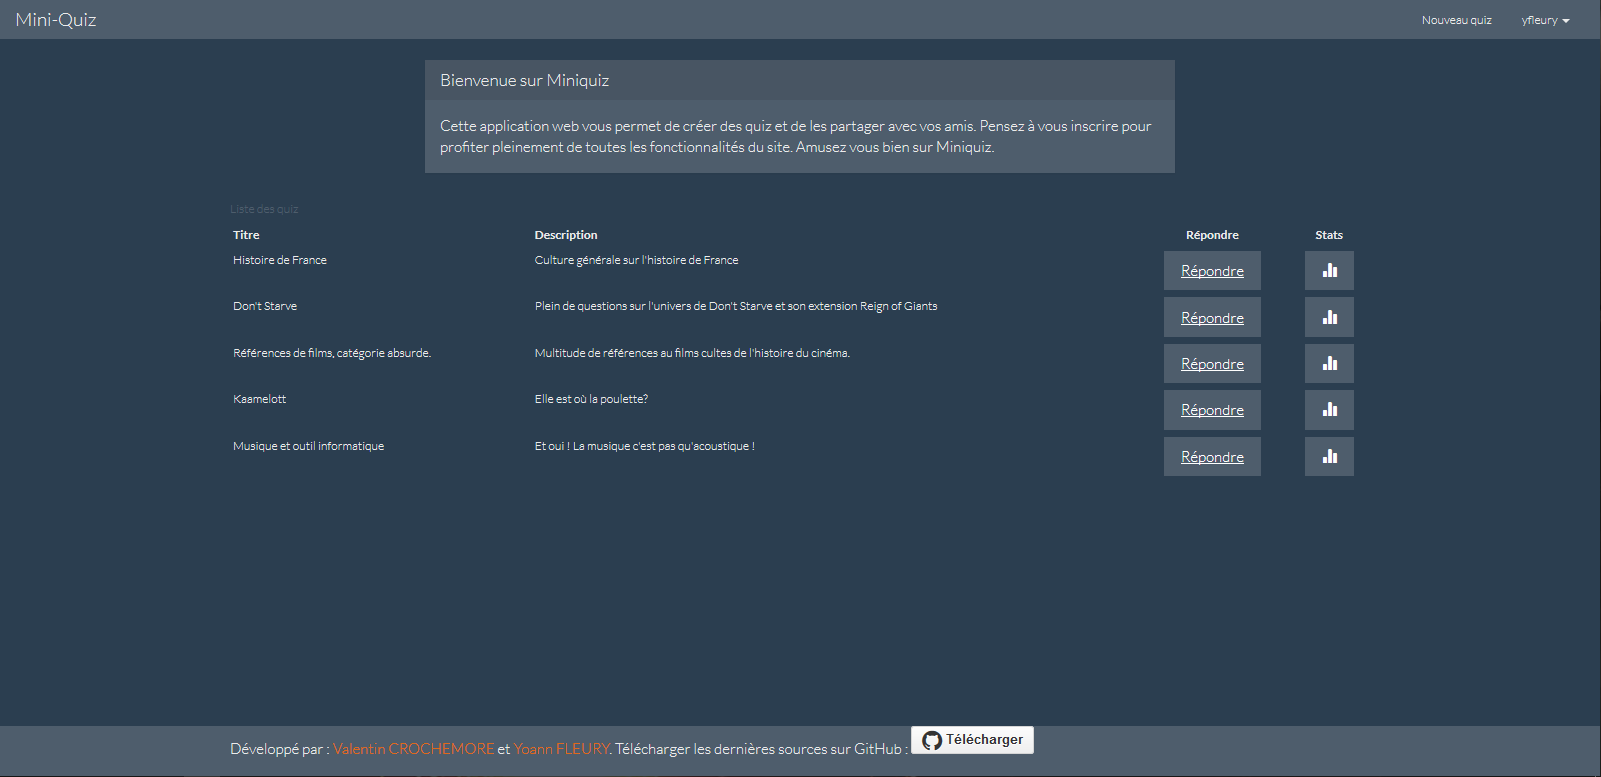
\includegraphics[width=\textwidth]{res/miniquiz-home.png}
        \end{figure}
        \begin{figure}[!ht]
            \caption{\label{fig:miniquiz-home-rwd} Capture de la page d'accueil de Miniquiz en responsive web design}
            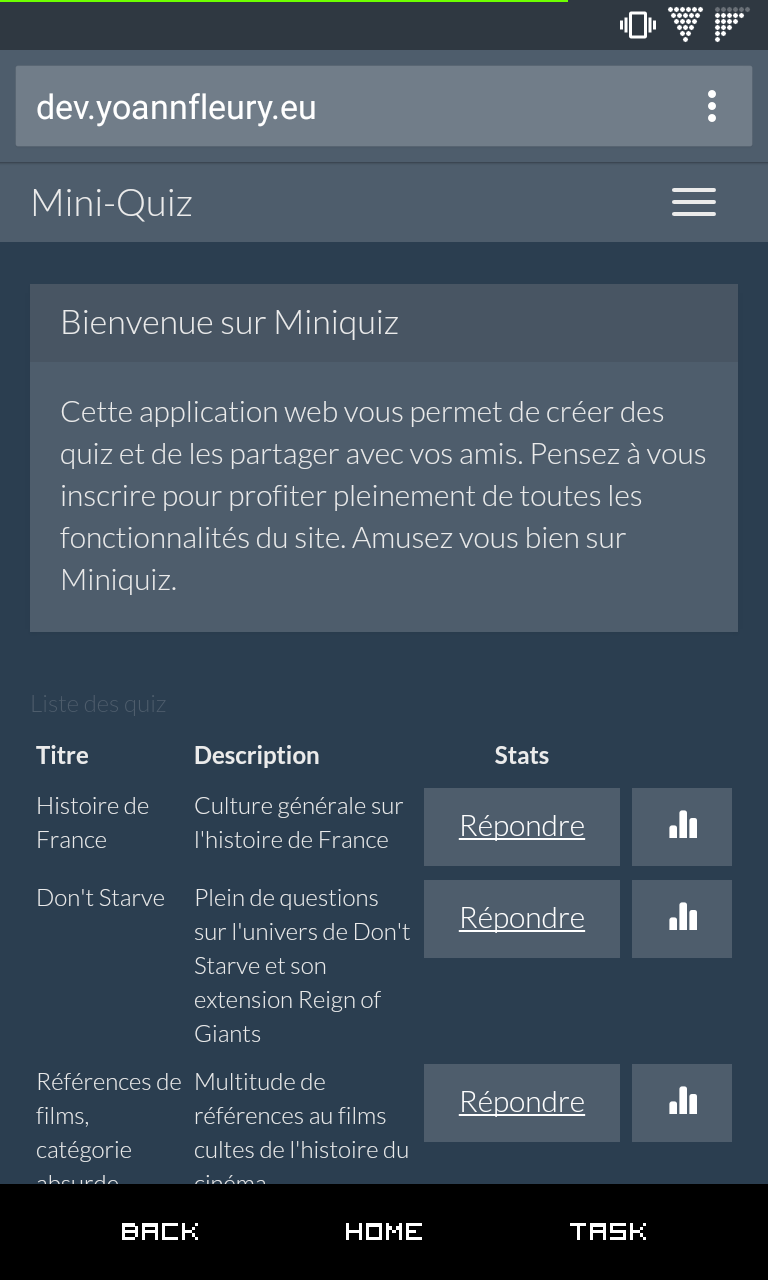
\includegraphics[scale=0.2]{res/miniquiz-home-rwd.png}
        \end{figure}
        \begin{figure}[!ht]
            \caption{\label{fig:miniquiz-question-rwd} Capture d'une question sur l'application Miniquiz}
            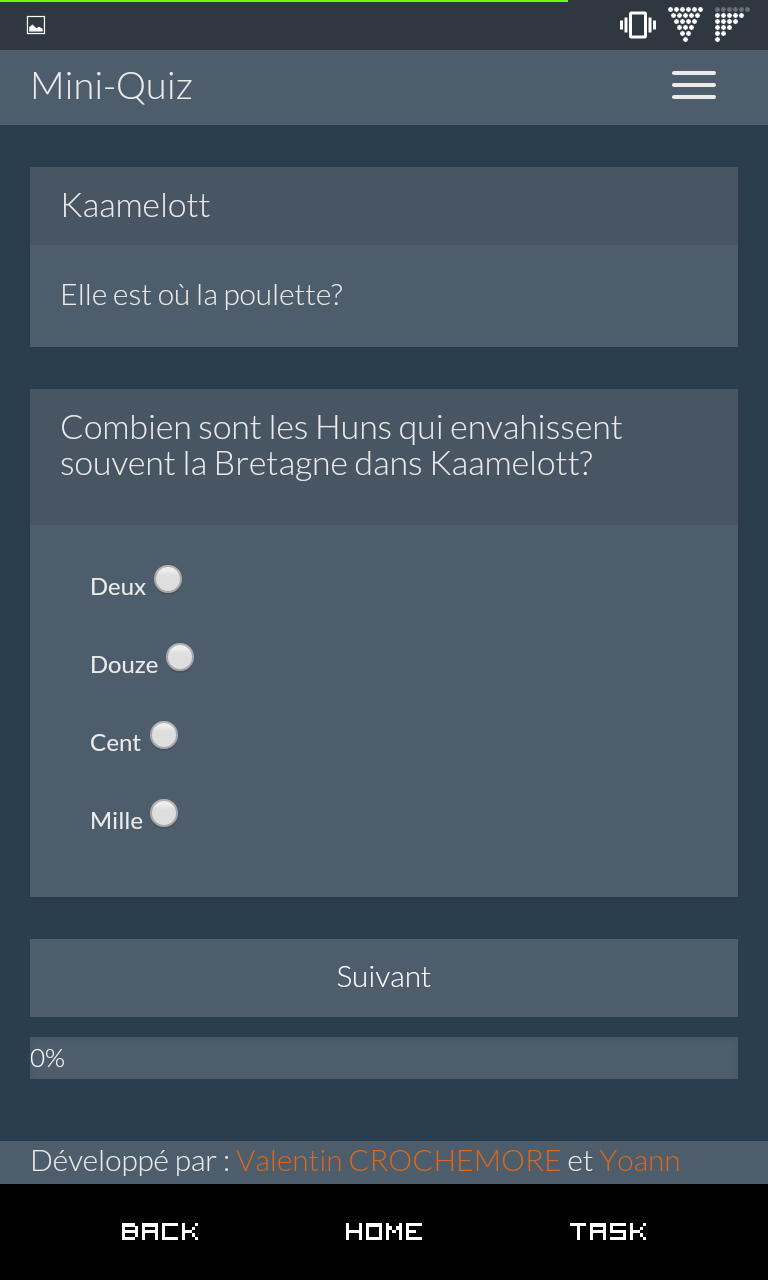
\includegraphics[scale=0.2]{res/miniquiz-question-rwd.png}
        \end{figure}
        \begin{figure}[!ht]
            \caption{\label{fig:miniquiz-progress-rwd} Capture d'une question sur l'application Miniquiz avec la barre de progression}
            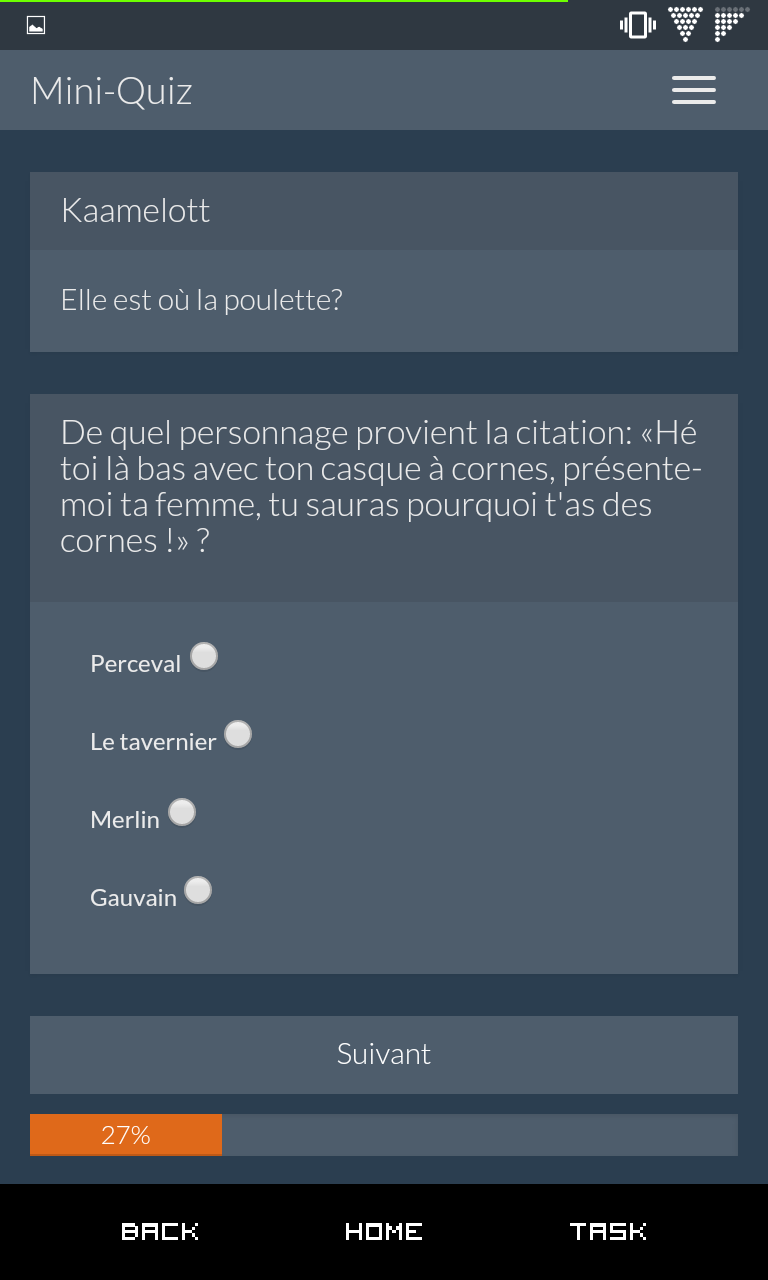
\includegraphics[scale=0.2]{res/miniquiz-progress-rwd.png}
        \end{figure}
    

\section{Installation}
    \paragraph{Instance} Vous pouvez dès maintenant accéder à \texttt{dev.yoannfleury.eu} pour rejoindre la communauté des Miniquizeurs sur une instance hébergée chez gandi.net. Vous pouvez voir les utilisateurs présents sur cette instance en accédant à la route \texttt{/users}.

    \paragraph{Conditions} Pour le bon fonctionnement de cette application, il faut les éléments suivant sur votre système :
    \begin{description}
        \item[curl] pour le bon fonctionnement du script d'installation
        \item[apache >= 2.4]
        \item[php >= 5.4] à la fois sur le serveur web et dans le PATH pour le script d'installation. Il faut également les extensions suivantes : \texttt{php5-cli}, \texttt{php5-curl} et \texttt{php5-json}
        \item[MySQL >= 5.6] pour la base de données. La commande \texttt{MySQL} doit également se trouver dans le PATH pour le script d'installation.
    \end{description}
    
    \paragraph{Installation via le script d'installation}
    \begin{enumerate}
        \item Téléchargez les sources de l'application grâce à la commande
        \begin{center}
            \texttt{git  clone https://github.com/yoannfleurydev/mini-quiz.git .}\\
        \end{center} 
        à la racine de votre serveur. Vous devez voir le fichier \texttt{install.php} à la racine de votre serveur web.
        \item Créez la base de donnée dans MySQL avec le nom que vous souhaitez. 
        \item Exécutez la commande  
        \begin{center}
            \texttt{php install.php}\\
        \end{center}
        et suivez les instructions.
        \item Complétez le fichier \texttt{app/config/prod.example.php} avec vos configurations et renommez ce fichier en \texttt{prod.php}.
        \item Vous pouvez maintenant accéder à Miniquiz. Amusez vous bien.
    \end{enumerate}
    
    \paragraph{Installation manuelle}
    \begin{enumerate}
        \item Téléchargez les sources de l'application grâce à la commande
        \begin{center}
            \texttt{git  clone https://github.com/yoannfleurydev/mini-quiz.git .}
        \end{center} 
        à la racine de votre serveur. Vous devez voir le fichier README.md à la racine de votre serveur. 
        \item Téléchargez Composer et installez les dépendances grâce à la commande 
        \begin{center}
            \texttt{php composer.phar install}
        \end{center}
        \item Dans MySQL créez la base de données à vide.
        \item Importez le script de création de base de données dans MySQL qui se trouve dans le dossier \texttt{db/}.
        \item Complétez le fichier \texttt{app/config/prod.example.php} avec vos configurations et renommez ce fichier en \texttt{prod.php}.
        \item Dans votre navigateur préféré (nous conseillons l'utilisation de Firefox), accédez à l'application. Inscrivez-vous pour créer le premier compte sur l'application. 
        \item Dans MySQL, mettez à jour l'utilisateur que vous venez de créer pour qu'il ait les droit d'administrateur, c'est à dire que vous devez mettre \texttt{user\_access\_id} à \texttt{1}.
        \item Vous pouvez maintenant utiliser Miniquiz en administrateur. Amusez vous bien sur Miniquiz.
    \end{enumerate}

\section{Bonnes pratiques et Sécurité}
    \paragraph{Bonnes pratiques} On pourrait citer dans les bonnes pratiques l'utilisation d'un framework qui permet de fixer des conventions, des normes de code, et qui formate un peu le développeur qui l'utilise. L'utilisation du MVC peut également être mentionné dans les bonnes pratiques. Nous avons suivi des conventions basiques comme le code en anglais, les routes en anglais, des concepts de programmation comme l'utilisation de DAO et de POPO.

    \paragraph{Sécurité} Au niveau de la sécurité, nous avons utilisé des concepts basiques comme l'utilisation de fonctions permettant le filtrage des entrées utilisateur comme \texttt{htmlspecialchars}. Pour les mots de passe, nous avons choisi d'utiliser la technique de hashage B\_CRYPT qui est selon les spécialistes en sécurité web le meilleur moyen de protéger un mot de passe actuellement.
    
    \paragraph{NTUI} Nous avons pris en compte le principe NTUI\footnote{Never Trust User Input} dans notre développement côté serveur. Grâce aux méthodes fournies par PHP, mais également grâce à nos propres tests.
    
    \paragraph{XSS} Nous avons également pris en compte les failles XSS\footnote{Cross-Site Scripting} de façon à suivre un maximum l'OWASP\footnote{Open Web Application Security Project}

\section{Ce que nous avons appris}
    \subsection{Problèmes rencontrés}
        \paragraph{SVG et MathML}Par manque de temps sur le projet, nous n'avons pas mis en place le système de réponse riches contenant du SVG ou du MathML. Pour le mettre en place, nos aurions utiliser un système de vérification grâce à une grammaire (DTD) qui défini le langage de balise pour le SVG ou le MathML.
        \paragraph{password\_hash()}Cette fonction n'est utilisable que sous PHP 5.5 il a donc fallu trouver un moyen d'assurer une compatibilité plus basse pour les serveurs qui n'utilisent pas une version si haute de PHP comme par exemple les instances \texttt{Simple Hosting} chez Gandi qui sont sous PHP 5.4 au moment ou on écrit ces lignes.
        
    \subsection{Nouvelles connaissances}
        \paragraph{}Grâce à ce projet, nous avons appris à utiliser le framework Silex, à construire un projet de A à Z en utilisant les dernières technologies du web comme Composer, Silex, et Bootstrap. 
        \paragraph{}L'utilisation de Silex nous a également permis de nous former à Symfony2 et à ces composants les plus basiques, ainsi qu'à l'utilisation de routes avec des paramètres.
    
\section{Sigles et terminologie}
    \begin{description}
        \item[CSS] Cascading StyleSheet.
        \item[DOM] Document Object Model. Interface indépendante de tout langage de programmation qui permet de manipuler du contenu HTML ou XML.
        \item[HTML] HyperText Markup Language. Langage de balises permettant une représentation sémantique de données.
        \item[NTUI] Never Trust User Input.
        \item[OWASP] Open Web Application Security Project.
        \item[URL] Uniform Resource Locator.
        \item[XSS] Cross-Site Scripting.
    \end{description}

\end{document}
